\subsection{Definition}
\begin{frame}{Popularity: Definition}
Since we are using MAL database and it has a social component, seems logic to use \emph{member\_favorites} as a representation of \emph{popularity}. We can also get popularity and score of anime from opinions of the same set of users.
\vspace{-10pt}

\begin{table}[!h]
	\begin{center}
	\begin{tabular}{|l|c|l|}
		\hline
		Name & Popularity & Some popular roles of them\\ 
		\hline
		Kana Hanazawa & 56637 & \textit{Angel Beats!}: Tachibana, Kanade \\
		\hline
		Hiroshi Kamiya & 49685 & \textit{Shingeki no Kyojin}: Levi, \\
		\hline
		Mamoru Miyano & 43942 & \textit{Death Note}: Yagami, Light \\ 
		\hline
		Rie Kugimiya & 31668 & \textit{Fullmetal Alchemist}: Elric, Alphonse \\ 
		\hline
		Jun Fukuyama & 26811 & \textit{Ao no Exorcist}: Okumura, Yukio \\ 
		\hline
		Miyuki Sawashiro & 26501 & \textit{Durarara!!}: Sturluson, Celty \\ 
		\hline
		Tomokazu Sugita & 24449 & \textit{Gintama}: Sakata, Gintoki \\
		\hline
		Daisuke Ono & 24080 & \textit{Durarara!!}: Heiwajima, Shizuo \\
		\hline
		Saori Hayami & 18322 & \textit{Owari no Seraph}: Hiiragi, Shinoa \\ 
		\hline
		Aya Hirano & 18094 & \textit{Fairy Tail}: Heartfilia, Lucy \\
		\hline
	\end{tabular}
	\end{center}
\end{table}
\end{frame}
%-------------------------------------------------------------------------

\subsection{Analysis}
\begin{frame}{Popularity: Analysis}
\begin{center}
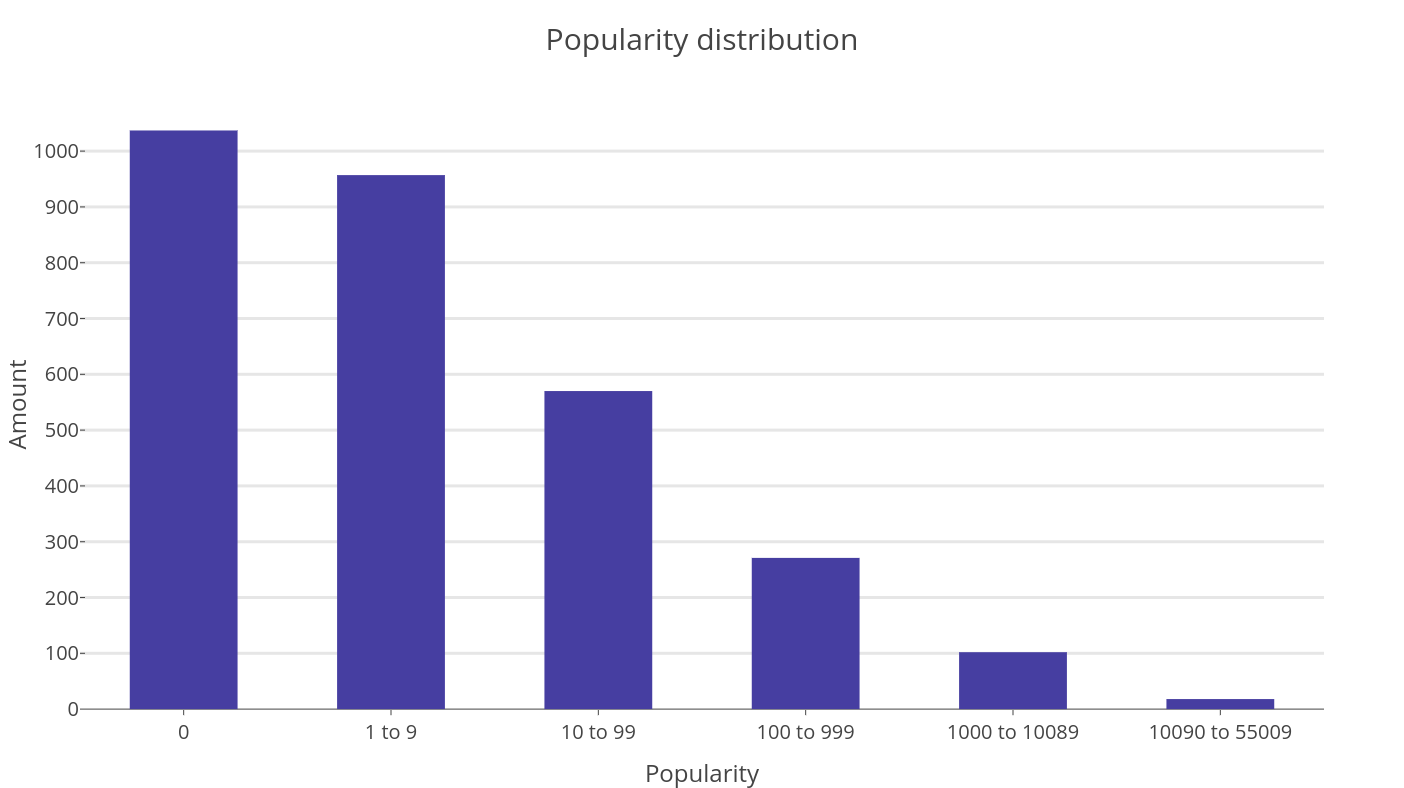
\includegraphics[scale=0.2]{graphics/popularityDistribution.png} 
\end{center}
\begin{table}[!htb]
    \begin{minipage}{.4\textwidth}
		\begin{itemize}
	\item Total: 2956
	\item Mean:    289.55
	\item Median:    2.0
		\end{itemize}
    \end{minipage}%
    \begin{minipage}{.6\textwidth}
        	\begin{itemize}
	\item Min:    0; Max:    55018
	\item 1037 values equal to zero
	\item Only 120 values bigger than 1000
		\end{itemize}
    \end{minipage}
\end{table}
\end{frame}
%-------------------------------------------------------------------------

\subsection{Pearson correlation}
\begin{frame}{Popularity: Pearson correlation}
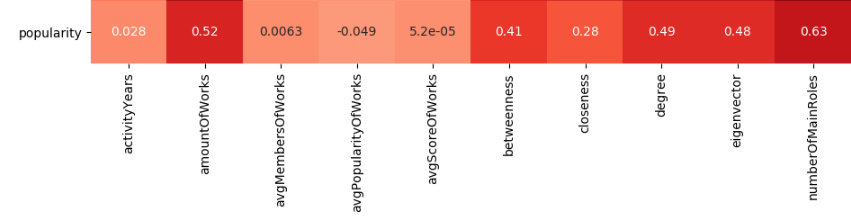
\includegraphics[scale=0.45]{graphics/popCorrelationAllWorks.png} 
\begin{itemize}
\item Big correlation between popularity and amount of works. %This attribute doesn't have the biggest correlation with popularity but "number of main roles" was added to the end of this investigation since we didn't had the data for doing so before. 
\item Number of main roles and amount of works have a strong correlation with each other (0.9) but they have different influence over popularity, this means they provide distinct information.
\end{itemize}

\end{frame}
%-------------------------------------------------------------------------

\begin{frame}
Since our dataset is biased in favor of more modern anime we thought of correlate with \emph{recent works} only.
\vspace{5pt}

But, how recent? Last 5, 10 or 20 years? 
\vspace{-5pt}

\begin{center}
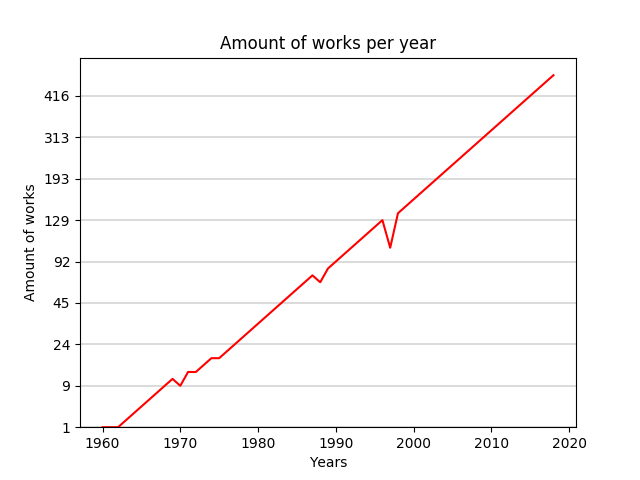
\includegraphics[scale=0.6]{graphics/worksPerYear_1960-2018.png} 
\end{center}

\end{frame}
%-------------------------------------------------------------------------

\begin{frame}
So our definition of recent works will be last 9 years.
\begin{center}
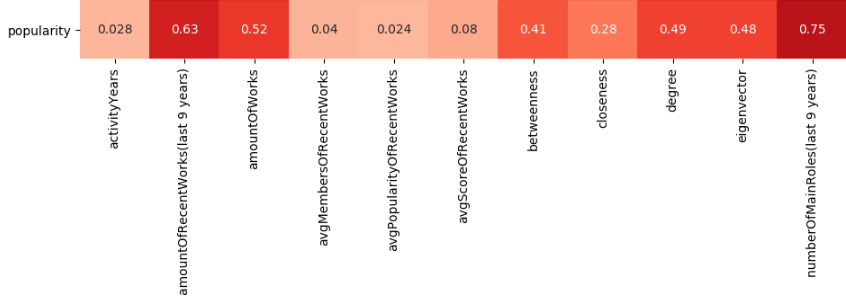
\includegraphics[scale=0.45]{graphics/popCorrelationRecentWorks.png} 
\end{center}
\begin{itemize}
\item Amount of recent works has more correlation with popularity than not recent.
\item It also happens with number of main roles.
\end{itemize}
\end{frame}
%-------------------------------------------------------------------------

\begin{frame}
Next graphs were made in order to discover \emph{why} \textit{9 years} prior had more correlation. 
\begin{figure}
	\centering
	\begin{subfigure}{.4\columnwidth}
		\centering
		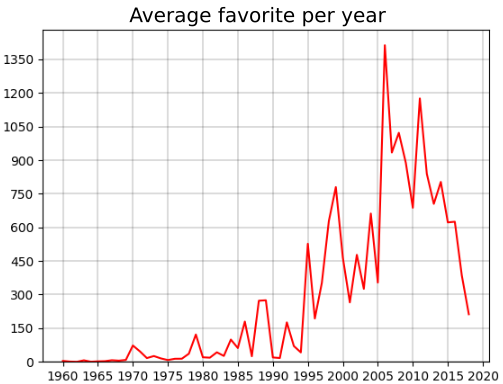
\includegraphics[width=\columnwidth]{graphics/avgFavorites.png}
	\end{subfigure}%
	\begin{subfigure}{.4\columnwidth}
		\centering
		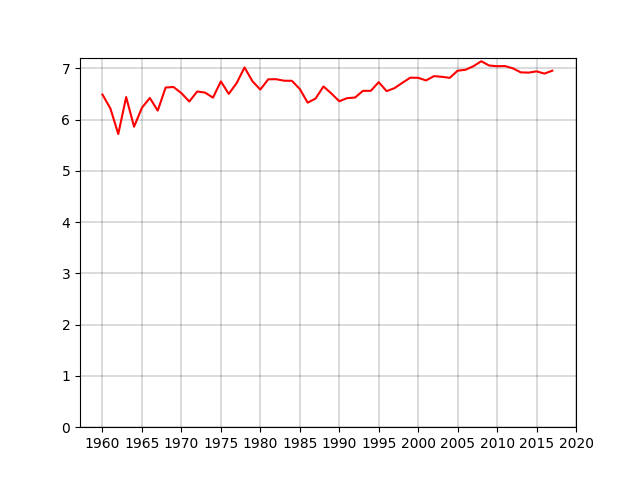
\includegraphics[width=\columnwidth]{graphics/avgScores.png}
	\end{subfigure}
	\begin{subfigure}{.4\columnwidth}
		\centering
		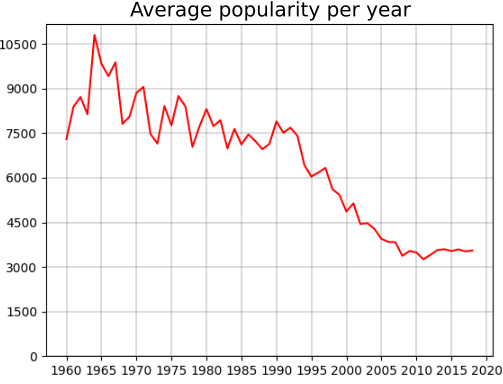
\includegraphics[width=\columnwidth]{graphics/avgPopularities.png}
	\end{subfigure}%
	\begin{subfigure}{.4\columnwidth}
		\centering
		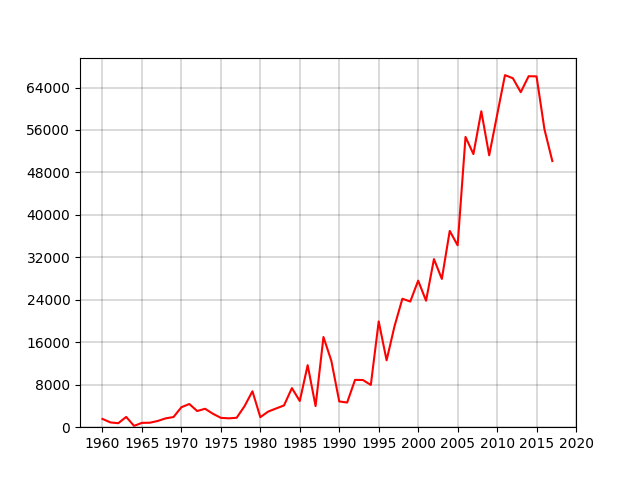
\includegraphics[width=\columnwidth]{graphics/avgMembers.png}
	\end{subfigure}
	\caption{Averages of favorites, score, popularity and amount of members.}
\end{figure}
\end{frame}
%-------------------------------------------------------------------------

\subsection{Prediction}
\begin{frame}{Popularity: Prediction}
The node attributes were divided into categories, leaving four distinct types:

\begin{figure}
	\centering
	\begin{subfigure}{.4\columnwidth}
		\begin{itemize}
			\item Personal data:
			\begin{itemize}
				\item Debut
				\item Gender
				\item Activity years (2018-debut)
			\end{itemize}
			\item Works data:
			\begin{itemize}
				\item Amount
				\item Top 5 genre
				\item Favorites
				\item Score
				\item Popularity
				\item Members
				\item Number of main roles
			\end{itemize}
		\end{itemize}
	\end{subfigure}%
	\begin{subfigure}{.6\columnwidth}
		\begin{itemize}
			\item Recent works data:
			\begin{itemize}
				\item Same as works but for only last 9 years
			\end{itemize}	
			\item Graph data:
			\begin{itemize}
				\item Degree
				\item Betweenness centrality
				\item Closeness
			\end{itemize}
		\end{itemize}
	\end{subfigure}
\end{figure}
\end{frame}
%-------------------------------------------------------------------------

\begin{frame}
Fitting and prediction experiments were run for each category, each combination of 2, 3 and all of them together; using Scikit-learn, 80\% of seiyuu as train data and the rest as test. This was done for all following models:
\begin{itemize}
	\item DecisionTreeRegressor
	\item DecisionTreeClassifier
	\item LinearRegression
	\item KNeighborsClassifier
	\item LinearDiscriminantAnalysis
	\item GaussianNB
	\item SVM
\end{itemize}
\end{frame}
%-------------------------------------------------------------------------

\begin{frame}
Because popularity variance is really high we got good results in metrics but particular predictions were aloof.
\vspace{5pt}

For example:\\
\emph{DecisionTreeClassifier} gets a r2\_score of 0.57 when using model data from \emph{works and recent works} categories but the scatter plot doesn't show such good results.
\vspace{-15pt}

\begin{figure}
	\begin{subfigure}{.5\columnwidth}
		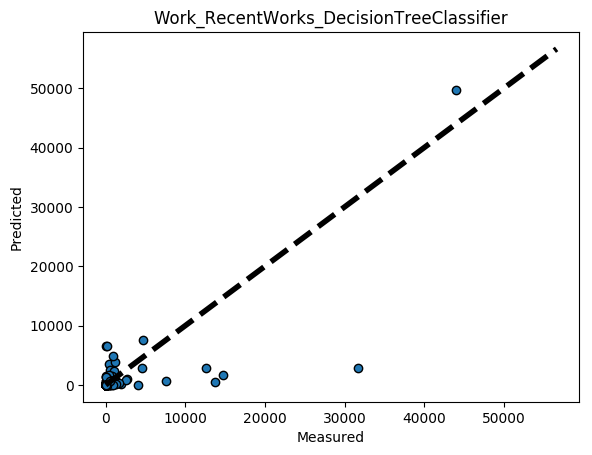
\includegraphics[scale=.36]{graphics/Work_RecentWorks_DecisionTreeClassifier.png} 
	\end{subfigure}%
	\begin{subfigure}{.5\columnwidth}
		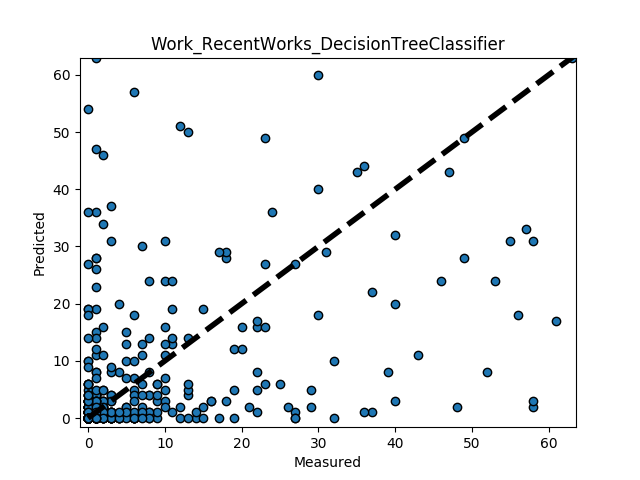
\includegraphics[scale=.4]{graphics/Work_RecentWorks_DecisionTreeClassifierZOOM.png} 
		\caption{Zoomed in}
	\end{subfigure}
\end{figure}

\end{frame}
%-------------------------------------------------------------------------

\begin{frame}{Popularity: Feature importance}
One of our goals about predicting popularity was to use the classifier algorithms to understand which are the key features that differentiates between a "not so much" and a popular seiyuu.
\vspace{5pt}

For our previous example we got:
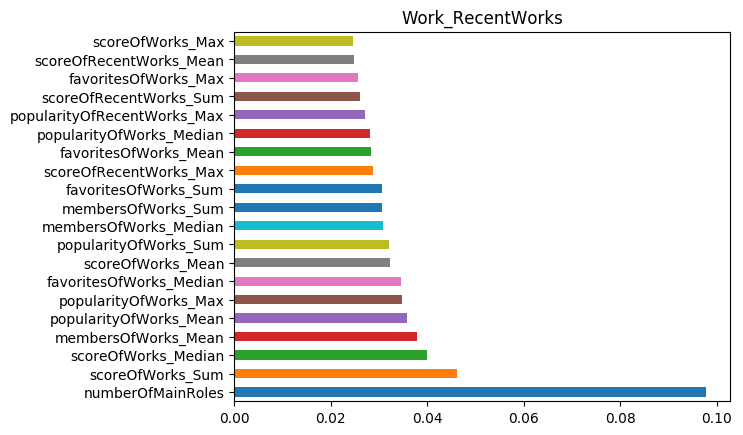
\includegraphics[scale=.5]{graphics/Work_RecentWorks_DTC_featureImportances.png} 

\end{frame}
%-------------------------------------------------------------------------